\documentclass[11pt,a4paper]{report}
\usepackage{tikz,graphicx}
\usepackage{titlesec}
\usepackage[utf8]{inputenc}
\usepackage[left=3.2cm,right=2.6cm]{geometry}
\usepackage{calc}
\usepackage{eso-pic}
\usepackage[section]{placeins}
\usepackage{float}
\usepackage[hidelinks]{hyperref}
\usepackage{listings}

\setlength{\topmargin}{0in}
\begin{document}


\title{Analysis of CPU Scheduling Algorithms}


\author{Kashish Srivastava (185014)\\
        \and 
        Dipesh Kumar (185015)\\
        \and
        Akash Rana (185034)
}

\titleformat{\chapter}{\bfseries\huge\centering}{}{0pt}{}{\huge}
\titlespacing*{\chapter}{0pt}{-60pt}{20pt}
\setlength{\parindent}{2em}
\setlength{\parskip}{1em}

\newenvironment{myindentpar}[1]%
  {\begin{list}{}%
          {\setlength{\leftmargin}{#1}}%
          \item[]%
  }
  {\end{list}}
\date{July 2020}

\pagestyle{plain}

\begin{titlepage}
    \begin{center}

        \Huge{\textbf{Analysis of CPU Scheduling Algorithms}}
 
        \vspace{5pt}
        
        \normalsize
       
        \vspace{5pt}
        
        Operating Systems\\
        CSD-222

    
        \vspace{10pt}
        
\includegraphics[width=0.4\textwidth]{./img/logo.png}
        
        \vspace{15pt}
        \textit{Submitted by:}
            Kashish Srivastava (185014)\\
            Dipesh Kumar (185015)\\
            Akash Rana (185034)
        \vspace{5pt}
 
        CSE (4 Year) : 
        4\textsuperscript{th} Semester
 
        \vspace{10pt}
 
        Under the guidance of
        
        \vspace{5pt}
        
        \textbf{Dr. Pradeep Singh }\\
		\large
		Assistant Professor\\ Department of Computer Science and Engineering\\
        National Institute of Technology, Hamirpur\\
      
    \end{center}
\end{titlepage}


\chapter{Introduction}
\vskip 1cm
This document is a report for the individual project ``Simulation of various CPU scheduling algorithms and analysing the behaviour of each scheduler". CPU scheduling is a process which allows one process to use the CPU while the execution of another process is on hold(in waiting state) due to unavailability of any resource like I/O etc, thereby making full use of CPU. The aim of CPU scheduling is to make the system efficient, fast and fair.\\ 
\vskip 1cm
\begin{figure}[H]
\centering
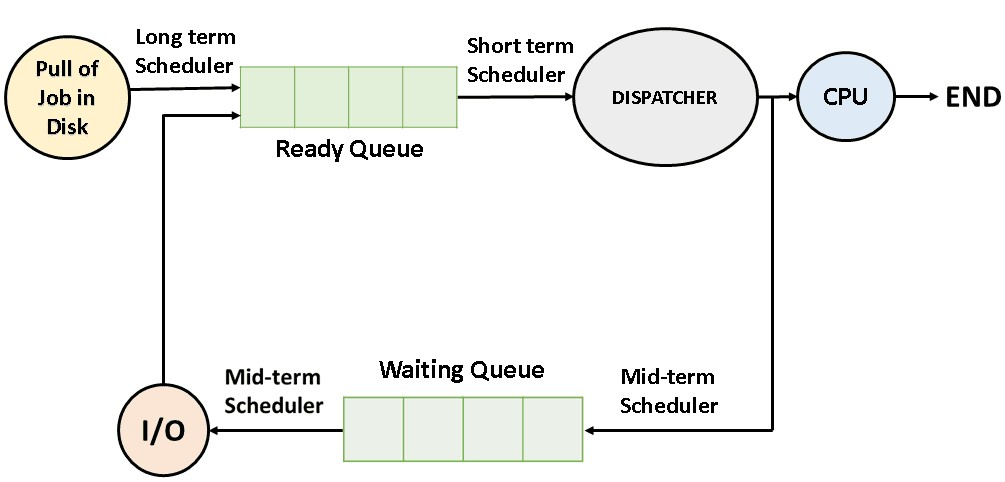
\includegraphics[scale=0.5]{./img/cpu.jpg}
\caption{Cpu scheduling}
\end{figure}

The project is an attempt to differentiate the behaviour of each scheduler with the statistical approach. In this project we performed each CPU scheduling and compared them on the basis of their completion time,throughput,average job elapsed time and average job waiting time during the process. It also discusses the complexity of the written code as instructed.


\chapter{Software requirement and specification}

\subsection*{Python(3.7.6)}
{Python is an interpreted, high-level, general-purpose programming language. Created by Guido van Rossum and first released in 1991, Python's design philosophy emphasizes code readability with its notable use of significant whitespace.}

{\subsection*{Python-dateutil(2.8.1)}
{The dateutil module provides powerful extensions to the standard datetime module, available in Python.}

\subsection*{matplotlib(3.2.2)}
{Matplotlib is a comprehensive library for creating static, animated, and interactive visualizations in Python.}

\subsection*{cycler(0.10.0)}
{A single entry Cycler object can be used to easily cycle over a single style.}


\subsection*{numpy(1.19.0)}
{NumPy is the fundamental package for scientific computing in Python. It is a Python library that provides a multidimensional array object, various derived objects (such as masked arrays and matrices).}

\subsection*{Kiwisolver(1.2.0)}
{Kiwisolver is an efficient C++ implementation of the Cassowary constraint solving algorithm. Kiwi is an implementation of the algorithm based on the seminal Cassowary paper.}

\subsection*{pyparsing(2.4.7)}
{Pyparsing is a mature, powerful alternative to regular expressions for parsing text into tokens and retrieving or replacing those tokens.}

\subsection*{six(1.15.0)}
{Six provides simple utilities for wrapping over differences between Python 2 and Python 3. It is intended to support codebases that work on both Python 2 and 3 without modification.}
}

\chapter{Usage}

Install Python 3.7.6 and then install all packages mentioned in 'requirements.txt' in root folder by:

	\begin{lstlisting}[ language=Python ]
		python -m pip install -r requirements.txt
		
	\end{lstlisting}

After Installing all the packages run the main script with command:

\begin{center}
	\begin{lstlisting}[ language=Python ]
		python main.py
		
	\end{lstlisting}
\end{center}


\begin{figure}[H]
\begin{center}
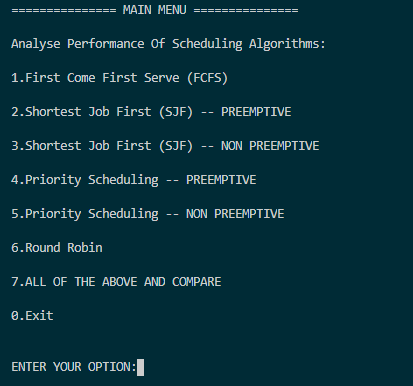
\includegraphics{./img/main.PNG}
\caption{Main Menu}
\label{fig}
\end{center}
\end{figure}



\tableofcontents

\chapter{First Come First Serve (FCFS)}


\begin{lstlisting}[language=Python,caption=fcfs source code]
import matplotlib.pyplot as plt

plt.style.use('fivethirtyeight')

## Finds waiting time for each process
def findWaitingTime(processes,  burst_time, waiting_time, arrival_time):  
    service_time = [0] *len(processes) 
    service_time[0] = 0
    waiting_time[0] = 0
    for i in range(1, len(processes)):  
           
        service_time[i] = (service_time[i - 1] +  burst_time[i - 1])  
  
        waiting_time[i] = service_time[i] - arrival_time[i]  
        if (waiting_time[i] < 0): 
            waiting_time[i] = 0
      

#Finds Turn Around Time for All processes
def findTurnAroundTime(processes, burst_time, waiting_time, turn_around_time):  
    for i in range(len(processes)): 
        turn_around_time[i] = burst_time[i] + waiting_time[i]  
  
  
#Returns waiting,turn around, completion time for each process
def findavgTime(processes,  burst_time, arrival_time):  

    waiting_time = [0] *len(processes)
    turn_around_time = [0] *len(processes) 
    findWaitingTime(processes,  burst_time, waiting_time, arrival_time)  
    findTurnAroundTime(processes,  burst_time, waiting_time, turn_around_time)  

    total_wt = 0
    total_turn_around_time = 0
    compl_time = [0]*len(processes)
    for i in range(len(processes)): 
  
        total_wt = total_wt + waiting_time[i]  
        total_turn_around_time = total_turn_around_time + turn_around_time[i]  
        # Calculate completion time

        compl_time[i] = turn_around_time[i] + arrival_time[i] 

    return waiting_time , turn_around_time ,compl_time


def plot_graph(processes,waiting_time,compl_time,turn_around_time):

    plt.plot(processes,waiting_time,label = "Waiting time")
    plt.plot(processes,compl_time,label = "Completion time")
    plt.plot(processes,turn_around_time,label = "Turnaround Time")
    plt.text(4,2,'Throughput = %.5f'  % (len(processes)/ compl_time[len(processes)-1]))
    plt.title("First Come First Serve Algo")
    plt.xlabel("Processes")
    plt.ylabel("Time Units")
    plt.legend()
    plt.savefig('./output/FCFS_output.png')
    plt.show()



def print_details(processes,waiting_time,turn_around_time,compl_time,burst_time,arrival_time):
      
    print("Processes   Burst Time   Arrival Time     Waiting",  
          "Time   Turn-Around Time  Completion Time \n") 
    for i in range(len(processes)):
        print(" ", processes[i] , "\t\t", burst_time[i], "\t\t", arrival_time[i],  
              "\t\t", waiting_time[i], "\t\t ", turn_around_time[i], "\t\t ", compl_time[i])  
  
    print("Average waiting time = %.5f "%(sum(waiting_time) /len(processes))) 
    print("\nAverage turn around time = ", sum(turn_around_time) / len(processes))  
    print('\nThroughput = ', len(processes)/ compl_time[len(processes)-1])


# driver function

def fcfs():
 
    processes = []
    burst_time = []
    arrival_time = []
    #breakpoint
    with open('./inputs/FCFS.txt','r') as  f:
        f.readline()
        for line in f.readlines():
            process , burst , arrival = (line.split(" "))
            processes.append(process)
            burst_time.append(int(burst))
            arrival_time.append(int(arrival))

    #returned waiting time and turn around time
    waiting_time , turn_around_time, compl_time = findavgTime(processes,  burst_time, arrival_time)
    
    #print details about data
    print_details(processes,waiting_time,turn_around_time,compl_time,burst_time,arrival_time)

    #plotting 
    plot_graph(processes,waiting_time,compl_time,turn_around_time)
    plt.close(fig='all')

if __name__ =="__main__": 
    fcfs()
\end{lstlisting}

\begin{figure}[H]
	\centering
	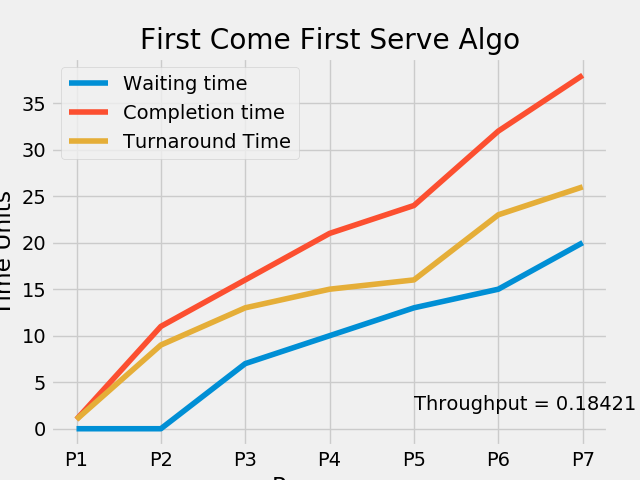
\includegraphics[scale=0.8]{./img/FCFS_output.png}
	\caption{FCFS output values.}
\end{figure}

\begin{figure}[H]
	\centering
	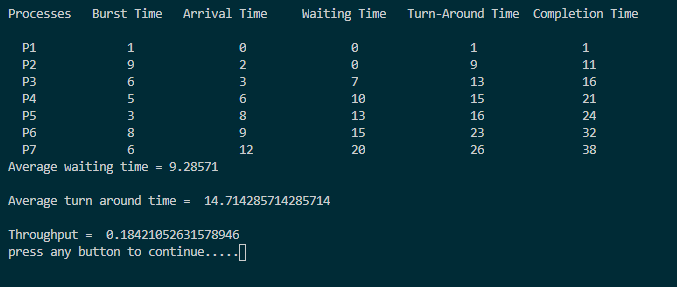
\includegraphics[scale=0.8]{./img/fcfs_out.PNG}
	\caption{FCFS output values.}
\end{figure}


\chapter{Shortest Job First(SJF)}
\section{SJF(Preemptive)}

{\begin{figure}[H]
	\centering
	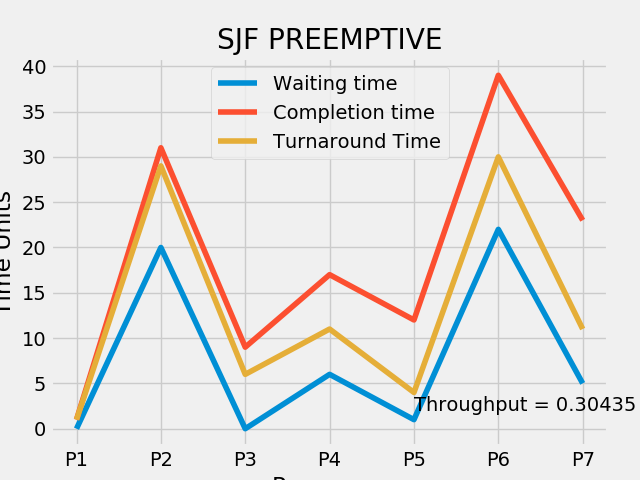
\includegraphics[scale=0.75]{./img/SJF_P_output.png}
	\caption{SJF(Preemptive) output values.}
\end{figure}}

{\begin{figure}[H]
	\centering
	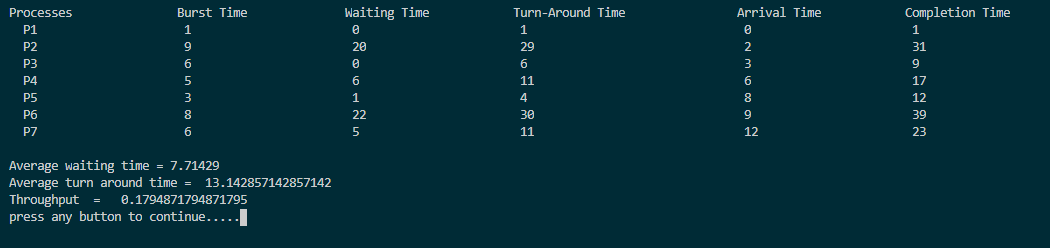
\includegraphics[scale=0.5]{./img/sjf_p_out.PNG}
	\caption{SJF(Preemptive) output values.}
\end{figure}}

\section{SJF(Non-Preemptive)}

{\begin{figure}[H]
	\centering
	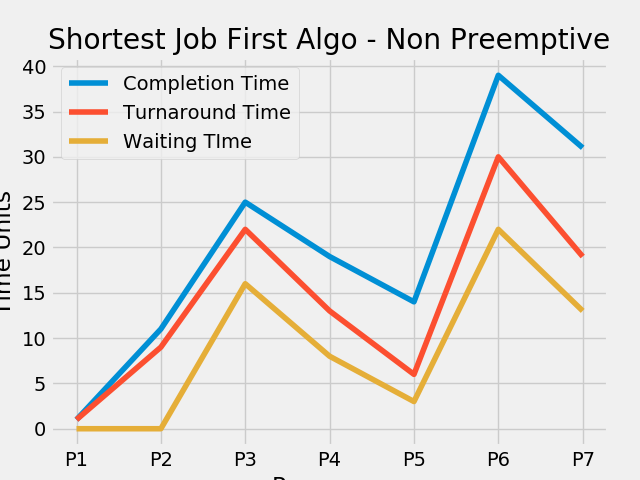
\includegraphics[scale=0.75]{./img/SJF_NP_output.png}
	\caption{SJF(Preemptive) output values.}
\end{figure}}

{\begin{figure}[H]
	\centering
	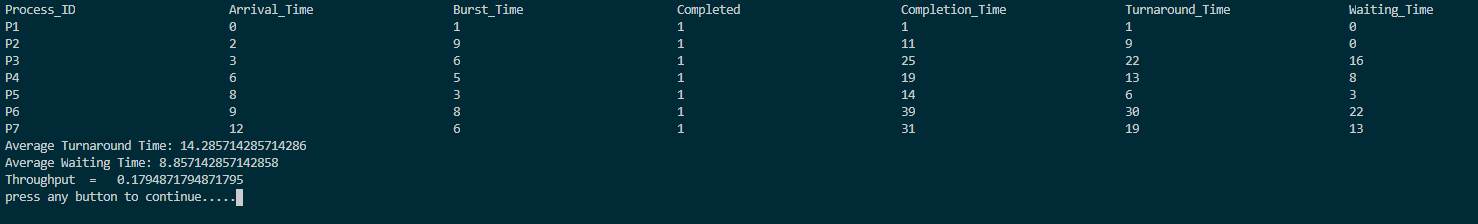
\includegraphics[scale=0.4]{./img/sjf_np_out.PNG}
	\caption{SJF(Preemptive) output values.}
\end{figure}}


\chapter{Priorty Scheduling}
\section{Priorty(Preemptive)}

{\begin{figure}[H]
	\centering
	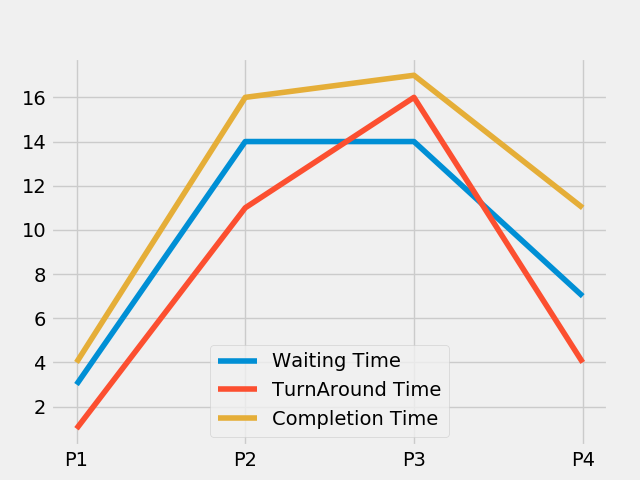
\includegraphics[scale=0.75]{./img/PRIORITY_P_output.png}
	\caption{SJF(Preemptive) output values.}
\end{figure}}

{\begin{figure}[H]
	\centering
	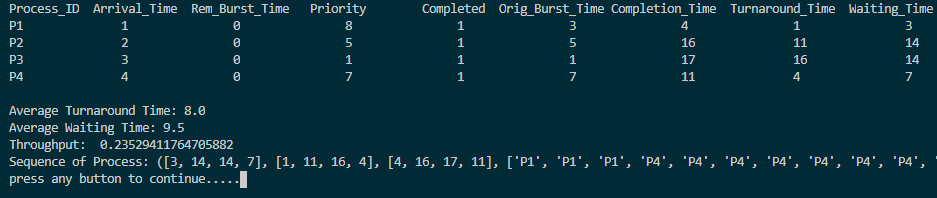
\includegraphics[scale=0.5]{./img/priority_p_out.PNG}
	\caption{SJF(Preemptive) output values.}
\end{figure}}

\section{Priorty(Non-Preemptive)}

{\begin{figure}[H]
	\centering
	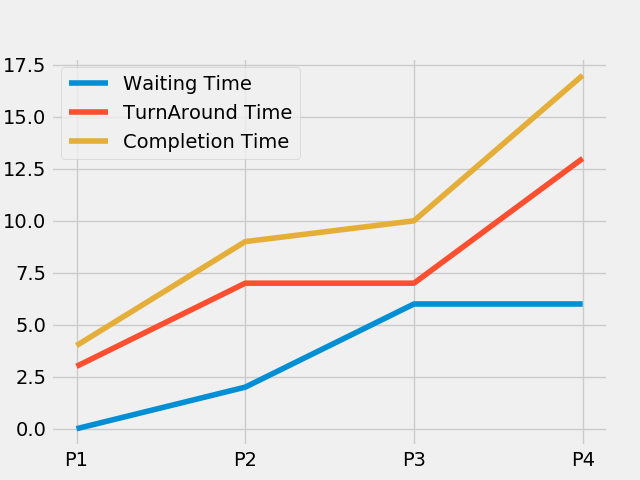
\includegraphics[scale=0.75]{./img/PRIORITY_NP_output.png}
	\caption{SJF(Preemptive) output values.}
\end{figure}}

{\begin{figure}[H]
	\centering
	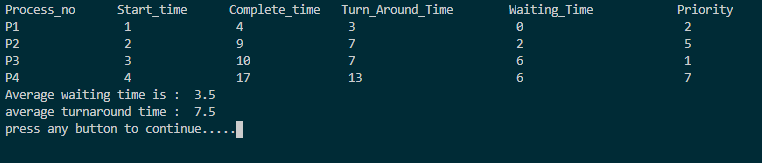
\includegraphics[scale=0.75]{./img/priority_np_out.PNG}
	\caption{SJF(Preemptive) output values.}
\end{figure}}


\chapter{Round Robin}

\begin{figure}[H]
	\centering
	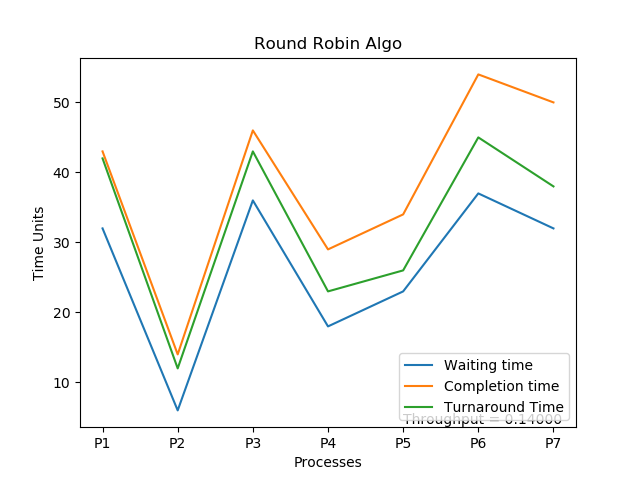
\includegraphics[scale=0.8]{./img/ROUND_ROBIN_output.png}
	\caption{FCFS output values.}
\end{figure}

\begin{figure}[H]

	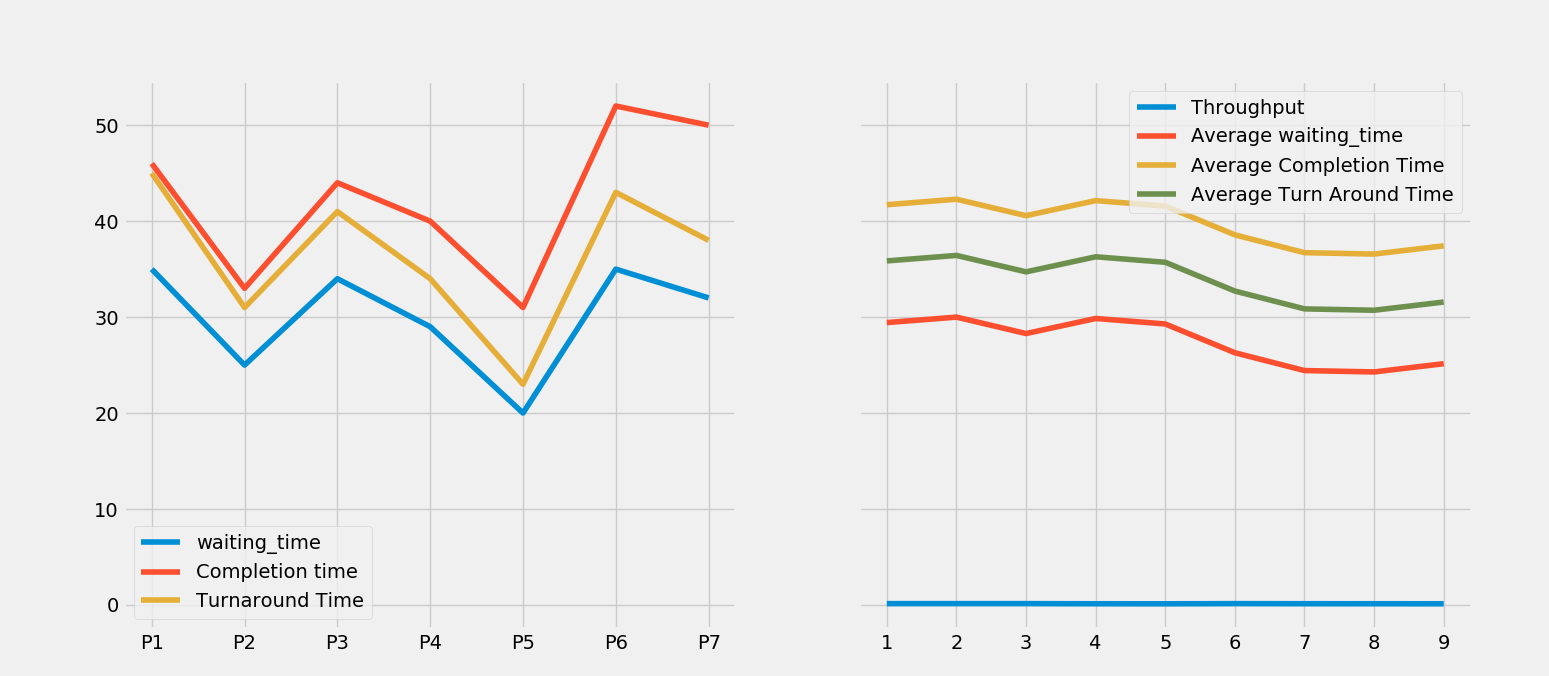
\includegraphics[scale=0.4]{./img/ROUND_ROBIN.png}
	\caption{FCFS output values.}
\end{figure}

\begin{figure}[H]

	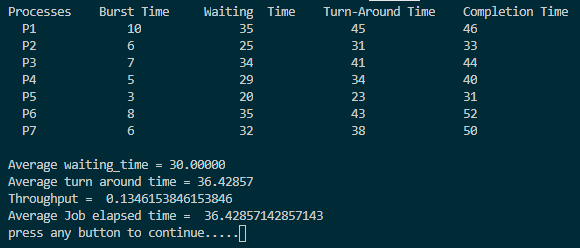
\includegraphics[scale=0.9]{./img/rr_out.PNG}
	\caption{FCFS output values.}
\end{figure}


\chapter{Conclusion}
\vskip 1cm
\large{{From the given project work we have concluded that the difference between the turn around time,average waiting time,average elapsed time and completion time for same input of different cpu scheduling is as follows:-}
\vskip 1cm
\begin{figure}[H]
	\centering
	\includegraphics[scale=0.9]{./img/compare.png}
	\caption{comparison between CPU scheduling.}
\end{figure}
\vskip 1cm
\large{from the above graph we came to know that every algorithm works better on the significant problem as the fcfs is better for a small burst time.The sjf is better if the process comes to processor simultaneously and round robin, is better to adjust the average waiting time desired and the priorty works better  where the relative important of each process may be precisely defined.}
}
\vskip 15cm

\chapter{References}
\vskip 1cm
{\subsection*{}
{\large{The source code of the project can be found at:-}\\
	\url{https://github.com/cannibalcheeseburger/cpu-scheduling-simluation.git}\\
\large{	And the other references we used for this project are given:-}
\begin{itemize}
\item 	A. Dusseau, R. H. dan A. C., Operating Systems: Three Easy Pieces, Arpaci-Dusseau Books, 2014.
\item Operating System Principles – Galvin
\item Tanenbaum, Modern Operating Systems, Pearson Education, Inc., 2008.
\item 	\url{http://www.cs.uic.edu/~jbell/CourseNotes/OperatingSystems/5_CPU_Scheduling.html}
\item \url{http://codex.cs.yale.edu/avi/os-book/OS8/os8c/slide-dir/PDF-dir/ch5.pdf}
\end{itemize}
}
}

\end{document}